\chapter{Appendix: Anforderungen}
\label{ch:appendix:requirements}
% Die folgenden Definitionen wurden wörtlich aus der ISO-Norm 25010 (\cite{ISO25010}) entnommen:
%
% \section*{functional suitability}
% "degree to which a product or system provides functions that meet stated and implied needs when used under specified conditions"
% \begin{description}
%   \item[functional completeness] "degree to which the set of functions covers all the specified tasks and user objectives"
%   \item[functional correctness] "degree to which a product or system provides the correct results with the needed degree of precision"
%   \item[functional appropriateness] "degree to which the functions facilitate the accomplishment of specified tasks and objectives"
% \end{description}
%
% \section*{performance efficiency}
% "performance relative to the amount of resources used under stated conditions"
% \begin{description}
%   \item[time behaviour] "degree to which the response and processing times and throughput rates of a product or system, when performing its functions, meet requirements"
%   \item[resource utilization] "degree to which the amounts and types of resources used by a product or system, when performing its functions, meet requirements"
%   \item[capacity] "degree to which the maximum limits of a product or system parameter meet requirements"
% \end{description}
%
% \section*{compatibility}
% "degree to which a product, system or component can exchange information with other products, systems or components, and/or perform its required functions, while sharing the same hardware or software environment"
% \begin{description}
%   \item[co-existence] "degree to which a product can perform its required functions efficiently while sharing a common environment and resources with other products, without detrimental impact on any other product"
%   \item[interoperability] "degree to which two or more systems, products or components can exchange information and use the information that has been exchanged"
% \end{description}
%
% \section*{usability}
% "degree to which a product or system can be used by specified users to achieve specified goals with effectiveness, efficiency and satisfaction in a specified context of use"
% \begin{description}
%   \item[appropriateness recognizability] "degree to which users can recognize whether a product or system is appropriate for their needs"
%   \item[learnability] "degree to which a product or system can be used by specified users to achieve specified goals of learning to use the product or system with effectiveness, efficiency, freedom from risk and satisfaction in a specified context of use"
%   \item[operability] "degree to which a product or system has attributes that make it easy to operate and control"
%   \item[user interface aesthetics] "degree to which a user interface enables pleasing and satisfying interaction for the user"
%   \item[accessibility] "degree to which a product or system can be used by people with the widest range of characteristics and capabilities to achieve a specified goal in a specified context of use"
% \end{description}
%
% \section*{reliability}
% "degree to which a system, product or component performs specified functions under specified conditions for a specified period of time"
% \begin{description}
%   \item[maturity] "degree to which a system, product or component meets needs for reliability under normal operation"
%   \item[availability] "degree to which a system, product or component is operational and accessible when required for use"
%   \item[fault tolerance] "degree to which a system, product or component operates as intended despite the presence of hardware or software faults"
%   \item[recoverability] "degree to which, in the event of an interruption or a failure, a product or system can recover the data directly affected and re-establish the desired state of the system"
%   \item[]
% \end{description}
%
% \section*{security}
% "degree to which a product or system protects information and data so that persons or other products or systems have the degree of data access appropriate to their types and levels of authorization"
% \begin{description}
%   \item[confidentiality] "degree to which a product or system ensures that data are accessible only to those authorized to have access"
%   \item[integrity] "degree to which a system, product or component prevents unauthorized access to, or modification of, computer programs or data"
%   \item[non-repudiation] "degree to which actions or events can be proven to have taken place, so that the events or actions cannot be repudiated later"
%   \item[accountability] "degree to which the actions of an entity can be traced uniquely to the entity"
%   \item[authenticity] "degree to which the identity of a subject or resource can be proved to be the one claimed"
% \end{description}
%
% \section*{maintainability}
% "degree of effectiveness and efficiency with which a product or system can be modified by the intended maintainers"
% \begin{description}
%   \item[modularity] "degree to which a system or computer program is composed of discrete components such that a change to one component has minimal impact on other components"
%   \item[reusability] "degree to which an asset can be used in more than one system, or in building other assets"
%   \item[analysability] "degree of effectiveness and efficiency with which it is possible to assess the impact on a product or system of an intended change to one or more of its parts, or to diagnose a product for deficiencies or causes of failures, or to identify parts to be modified"
%   \item[modifiability] "degree to which a product or system can be effectively and efficiently modified without introducing defects or degrading existing product quality"
%   \item[testability] "degree of effectiveness and efficiency with which test criteria can be established for a system, product or component and tests can be performed to determine whether those criteria have been met"
% \end{description}
%
% \section*{portability}
% "degree of effectiveness and efficiency with which a system, product or component can be transferred from one hardware, software or other operational or usage environment to another"
% \begin{description}
%   \item[adaptability] "degree to which a product or system can effectively and efficiently be adapted for different or evolving hardware, software or other operational or usage environments"
%   \item[installability] "degree of effectiveness and efficiency with which a product or system can be successfully installed and/or uninstalled in a specified environment"
%   \item[replaceability] degree to which a product can replace another specified software product for the same purpose in the same environment
% \end{description}


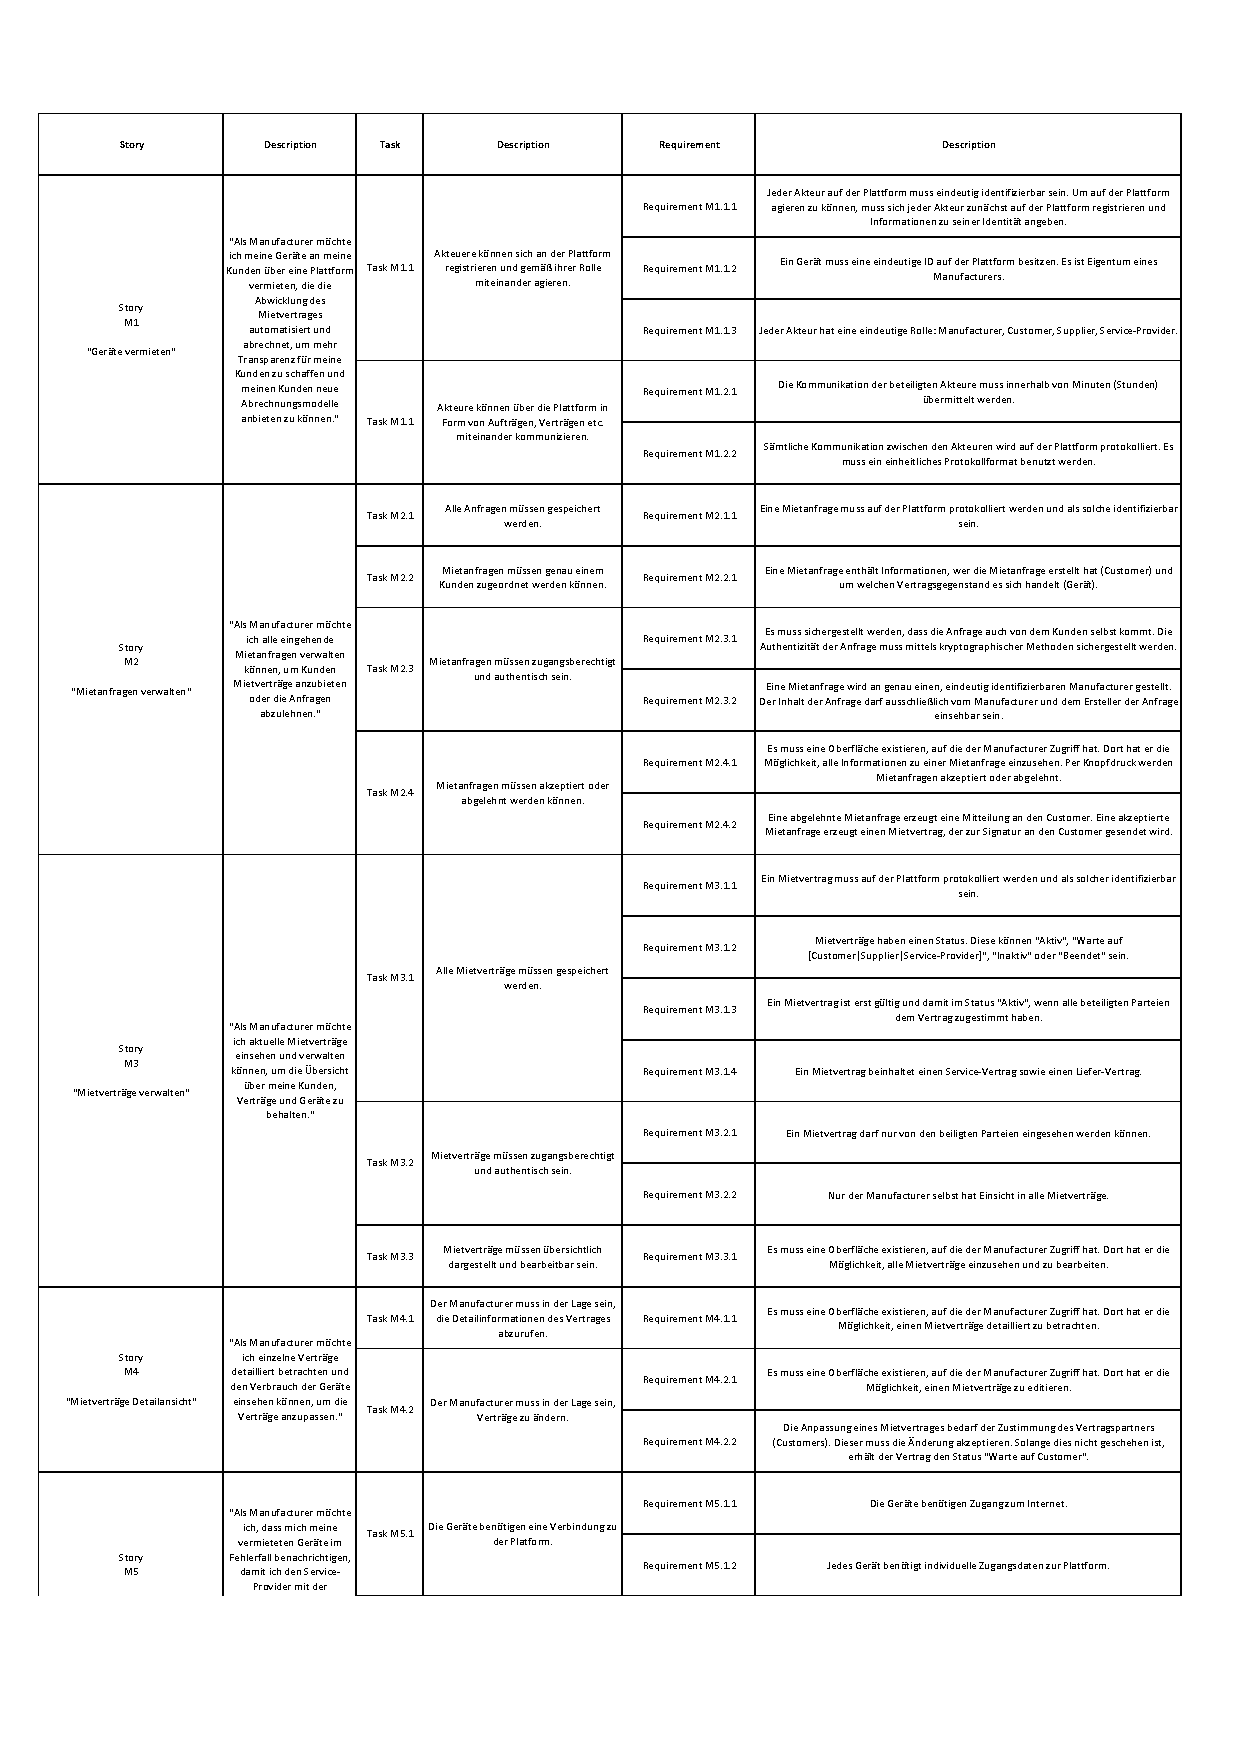
\includepdf[pages=-]{gfx/Requirements_v1.pdf}


% \graffito{
% \small
% Legende\\
% \tiny
% \textcolor{MidnightBlue!75!black}{\ding{110}} Manufacturer\\
% \textcolor{BrickRed!75!black}{\ding{110}} Customer\\
% \textcolor{Aquamarine!75!black}{\ding{110}} Service-Provider\\
% \textcolor{SpringGreen!75!black}{\ding{110}} Supplier\\
% \textcolor{Goldenrod!75!black}{\ding{110}} Platform-Operator\\
% \textcolor{DarkOrchid!75!black}{\ding{110}} Developer\\
% }
%
% %%%Manufacturer%%%
%
% \begin{tcolorbox}[colback=white,colframe=MidnightBlue!50!black, colbacktitle=MidnightBlue!75!black,title=\textbf{\underline{M1} Geräte vermieten}]
%   \label{req:m1}
%   \glqq Als Manufacturer möchte ich beliebig viele meiner Geräte an beliebig viele Kunden vermieten um Umsatz zu machen. \grqq
%   \tcblower
%   \begin{tcolorbox}[colback=white,colframe=white!50!black, colbacktitle=white!75!black,title=Task M1.1]
%     Die Platform muss so skalieren, sodass mehrere hunderttausend Geräte, einige tausend Kunden sowie Supplier und Service-Provider im unteren zweistelligen Bereich auf der Platform agieren können.
%   \end{tcolorbox}
%   \begin{tcolorbox}[colback=white,colframe=white!50!black, colbacktitle=white!75!black,title=Task M1.2]
%     Die Kommunikation der beteiligten Parteien (Aufträge, Mietverträge, Verbrauch, etc.) muss innerhalb von Minuten bzw. innerhalb von Stunden übermittelt werden.
%   \end{tcolorbox}
% \end{tcolorbox}
%
% \begin{tcolorbox}[colback=white,colframe=MidnightBlue!50!black, colbacktitle=MidnightBlue!75!black,title=\textbf{\underline{M2} Mietanfragen verwalten}]
%   \label{req:m2}
%   \glqq Als Manufacturer möchte ich alle eingehende Mietanfragen verwalten können, um Kunden Mietverträge anzubieten oder die Anfragen abzulehnen. \grqq
%   \tcblower
%   \begin{tcolorbox}[colback=white,colframe=white!50!black, colbacktitle=white!75!black,title=Task M2.1]
%     Alle Anfragen müssen gespeichert werden.
%   \end{tcolorbox}
%   \begin{tcolorbox}[colback=white,colframe=white!50!black, colbacktitle=white!75!black,title=Task M2.2]
%     Mietanfragen müssen genau einem Kunden zugeordnet werden können.
%   \end{tcolorbox}
%   \begin{tcolorbox}[colback=white,colframe=white!50!black, colbacktitle=white!75!black,title=Task M2.3]
%     Es muss sichergestellt werden, dass die Anfrage auch von dem Kunden selbst kommt.
%   \end{tcolorbox}
% \end{tcolorbox}
%
% \begin{tcolorbox}[colback=white,colframe=MidnightBlue!50!black, colbacktitle=MidnightBlue!75!black,title=\textbf{\underline{M3} Mietverträge verwalten}]
%   \label{req:m3}
%   \glqq Als Manufacturer möchte ich aktuelle Mietverträge einsehen und verwalten können, um die Übersicht über meine Kunden, Verträge und Geräte zu behalten. \grqq
%   \tcblower
%   \begin{tcolorbox}[colback=white,colframe=white!50!black, colbacktitle=white!75!black,title=Task M3.1]
%     Mietverträge dürfen nur für den Manufacturer selbst sichtbar sein.
%   \end{tcolorbox}
% \end{tcolorbox}
%
% \begin{tcolorbox}[colback=white,colframe=MidnightBlue!50!black, colbacktitle=MidnightBlue!75!black,title=\textbf{\underline{M4} Mietverträge Detailansicht}]
%   \label{req:m4}
%   \glqq Als Manufacturer möchte ich einzelne Verträge detailliert betrachten und den Verbrauch der Geräte einsehen können, um die Verträge anzupassen. \grqq
%   \tcblower
%   \begin{tcolorbox}[colback=white,colframe=white!50!black, colbacktitle=white!75!black,title=Task M4.1]
%     Der Manufacturer muss in der Lage sein, die Detailinformationen des Vertrages abzurufen.
%   \end{tcolorbox}
%   \begin{tcolorbox}[colback=white,colframe=white!50!black, colbacktitle=white!75!black,title=Task M4.2]
%     Der Manufacturer muss in der Lage sein, Verträge zu ändern. Die Änderung befarf der Zustimmung des Customers.
%   \end{tcolorbox}
% \end{tcolorbox}
%
% \begin{tcolorbox}[colback=white,colframe=MidnightBlue!50!black, colbacktitle=MidnightBlue!75!black,title=\textbf{\underline{M5} Benachrichtigung im Fehlerfall}]
%   \label{req:m5}
%   \glqq Als Manufacturer möchte ich, dass mich meine vermieteten Geräte im Fehlerfall benachrichtigen, damit ich den Service-Provider mit der Durchführung des Service beauftragen kann. \grqq
%   \tcblower
%   \begin{tcolorbox}[colback=white,colframe=white!50!black, colbacktitle=white!75!black,title=Task M5.1]
%     Die Geräte benötigen eine Verbindung zu der Platform.
%   \end{tcolorbox}
%   \begin{tcolorbox}[colback=white,colframe=white!50!black, colbacktitle=white!75!black,title=Task M5.2]
%     Die Geräte benötigen Sensoren, um Fehler und Defekte zu detektieren.
%   \end{tcolorbox}
% \end{tcolorbox}
%
% \begin{tcolorbox}[colback=white,colframe=MidnightBlue!50!black, colbacktitle=MidnightBlue!75!black,title=\textbf{\underline{M6} Abrechnung}]
%   \label{req:m6}
%   \glqq Als Manufacturer benötige ich eine korrekte, nutzungsabhängige und automatische Abrechnung der vermieteten Geräte, die täglich (stündlich) aktualisiert wird, um den Umsatz aufrecht zu erhalten. \grqq
%   \tcblower
%   \begin{tcolorbox}[colback=white,colframe=white!50!black, colbacktitle=white!75!black,title=Task M6.1]
%     Die Geräte benötigen Sensoren, um den Verbrauch zu detektieren.
%   \end{tcolorbox}
%   \begin{tcolorbox}[colback=white,colframe=white!50!black, colbacktitle=white!75!black,title=Task M6.2]
%     Die Geräte müssen die Verbrauchsdaten sammeln und aggregieren und in einem festgelegten Zeitintervall an die Platform melden.
%   \end{tcolorbox}
%   \begin{tcolorbox}[colback=white,colframe=white!50!black, colbacktitle=white!75!black,title=Task M6.3]
%     Es muss sichergestellt werden, dass die Verbrauchsdaten manipulationssicher von den Geräten selbst an die Platform gesendet werden.
%   \end{tcolorbox}
% \end{tcolorbox}
%
% \begin{tcolorbox}[colback=white,colframe=MidnightBlue!50!black, colbacktitle=MidnightBlue!75!black,title=\textbf{\underline{M7} Service-Provider beauftragen}]
%   \label{req:m7}
%   \glqq Als Manufacturer möchte ich aus einer Liste verfügbarer Service-Provider auswählen und diese beauftragen können, um meine vermieteten Geräte zu warten und zu reparieren. \grqq
%   \tcblower
%   \begin{tcolorbox}[colback=white,colframe=white!50!black, colbacktitle=white!75!black,title=Task M7.1]
%     Es muss eine Auflistung aller verfügbarer Service-Provider existieren.
%   \end{tcolorbox}
%   \begin{tcolorbox}[colback=white,colframe=white!50!black, colbacktitle=white!75!black,title=Task M7.2]
%     Eine Beauftragung eines Service-Providers bedarf dessen Zustimmung.
%   \end{tcolorbox}
%   \begin{tcolorbox}[colback=white,colframe=white!50!black, colbacktitle=white!75!black,title=Task M7.3]
%     Die Beauftragung muss alle benötigen Informationen über das Gerät, die Bezahlung, den Standort und den Defekt enthalten.
%   \end{tcolorbox}
% \end{tcolorbox}
%
% \begin{tcolorbox}[colback=white,colframe=MidnightBlue!50!black, colbacktitle=MidnightBlue!75!black,title=\textbf{\underline{M8} Service-Aufträge einsehen}]
%   \label{req:m8}
%   \glqq Als Manufacturer möchte ich den Status und die Kosten aktuell laufender Service-Aufträge einsehen können, um einen Überblick über meine offenden Aufträge behalten zu können. \grqq
%   \tcblower
%   \begin{tcolorbox}[colback=white,colframe=white!50!black, colbacktitle=white!75!black,title=Task M8.1]
%     This is a description.
%   \end{tcolorbox}
% \end{tcolorbox}
%
% \begin{tcolorbox}[colback=white,colframe=MidnightBlue!50!black, colbacktitle=MidnightBlue!75!black,title=\textbf{\underline{M9} Lierferungen beauftragen}]
%   \label{req:m9}
%   \glqq Als Manufacturer möchte ich aus einer Liste verfügbarer Supplier auswählen und diese beauftragen können, um meine vermieteten Geräte auszuliefern. \grqq
%   \tcblower
%   \begin{tcolorbox}[colback=white,colframe=white!50!black, colbacktitle=white!75!black,title=Task M9.1]
%     Es muss eine Auflistung aller verfügbarer Supplier existieren.
%   \end{tcolorbox}
%   \begin{tcolorbox}[colback=white,colframe=white!50!black, colbacktitle=white!75!black,title=Task M9.2]
%     Eine Lieferanfrage muss vom Supplier zunächst bestätigt werden; die Anfrage muss alle relevanten Informationen wie Standorte, Gerätemaße, etc. enthalten.
%   \end{tcolorbox}
% \end{tcolorbox}
%
% \begin{tcolorbox}[colback=white,colframe=MidnightBlue!50!black, colbacktitle=MidnightBlue!75!black,title=\textbf{\underline{M10} Lieferaufträge einsehen}]
%   \label{req:m10}
%   \glqq Als Manufacturer möchte ich den Status und die Kosten aktuell laufender Lieferaufträge einsehen können, um einen Überblick über meine offenen Aufträge behalten zu können. \grqq
%   \tcblower
%   \begin{tcolorbox}[colback=white,colframe=white!50!black, colbacktitle=white!75!black,title=Task M10.1]
%     This is a description.
%   \end{tcolorbox}
% \end{tcolorbox}
%
% %%%Customer%%%
%
% \begin{tcolorbox}[colback=white,colframe=BrickRed!50!black, colbacktitle=BrickRed!75!black,title=\textbf{\underline{C1} Ansicht verfügbarer Geräte}]
%   \label{req:c1}
%   \glqq Als Customer möchte ich verfügbare Haushaltsgeräte angezeigt bekommen, um das passende Gerät mieten zu können. \grqq
%   \tcblower
%   \begin{tcolorbox}[colback=white,colframe=white!50!black, colbacktitle=white!75!black,title=Task C1.1]
%     Es muss eine Auflistung aller verfügbarer (mietbarer) Geräte existieren.
%   \end{tcolorbox}
%   \begin{tcolorbox}[colback=white,colframe=white!50!black, colbacktitle=white!75!black,title=Task C1.2]
%     Es muss sichergestellt werden, dass sich das verfügbare Gerät in keinem Mietverhältnis befindet.
%   \end{tcolorbox}
%   \begin{tcolorbox}[colback=white,colframe=white!50!black, colbacktitle=white!75!black,title=Task C1.3]
%     Es müssen alle für den Customer relevaten Informationen über das Gerät vorhanden und einsehbar sein.
%   \end{tcolorbox}
% \end{tcolorbox}
%
% \begin{tcolorbox}[colback=white,colframe=BrickRed!50!black, colbacktitle=BrickRed!75!black,title=\textbf{\underline{C2} Überblick Mietverträge}]
%   \label{req:c2}
%   \glqq Als Customer möchte ich meine laufenden Mietverträge einsehen können, um den Überblick über meine aktuellen Kosten und Verbrauch behalten zu können. \grqq
%   \tcblower
%   \begin{tcolorbox}[colback=white,colframe=white!50!black, colbacktitle=white!75!black,title=Task C2.1]
%     Es muss sichergestellt werden, dass der Customer nur seine eigenen Mietverträge einsehen kann.
%   \end{tcolorbox}
%   \begin{tcolorbox}[colback=white,colframe=white!50!black, colbacktitle=white!75!black,title=Task C2.2]
%     Der Verbrauch und die Kosten (über einen Zeitraum X) müssen gespeichert und aufsummiert dargestellt werden.
%   \end{tcolorbox}
% \end{tcolorbox}
%
% \begin{tcolorbox}[colback=white,colframe=BrickRed!50!black, colbacktitle=BrickRed!75!black,title=\textbf{\underline{C3} Anpassung Mietvertrag}]
%   \label{req:c3}
%   \glqq Als Customer möchte ich einen laufenden Mietverträge bearbeiten können, um diesen kündigen oder weitere Geräte hinzubuchen zu können. \grqq
%   \tcblower
%   \begin{tcolorbox}[colback=white,colframe=white!50!black, colbacktitle=white!75!black,title=Task C3.1]
%     Es muss sichergestellt werden, dass ein Customer nur seine eigenen Verträge einsehen und bearbeiten kann.
%   \end{tcolorbox}
%   \begin{tcolorbox}[colback=white,colframe=white!50!black, colbacktitle=white!75!black,title=Task C3.2]
%     Ein Customer muss sich als er selbst authentifizieren können.
%   \end{tcolorbox}
% \end{tcolorbox}
%
% \begin{tcolorbox}[colback=white,colframe=BrickRed!50!black, colbacktitle=BrickRed!75!black,title=\textbf{\underline{C4} Geräte warten}]
%   \label{req:c4}
%   \glqq Als Customer möchte ich die gemieteten Geräte reinigen und warten können, um dafür vom Hersteller eine Gutschrift auf mein Vertragskonto zu erhalten. \grqq
%   \tcblower
%   \begin{tcolorbox}[colback=white,colframe=white!50!black, colbacktitle=white!75!black,title=Task C4.1]
%     Das Gerät muss die Reinigung / Wartung durch den Customer detektieren können.
%   \end{tcolorbox}
%   \begin{tcolorbox}[colback=white,colframe=white!50!black, colbacktitle=white!75!black,title=Task C4.2]
%     Es muss sichergestellt werden, dass eine Reinigung / Reparatur dem Gerät bzw. dessen Sensoren nicht vorgespielt werden kann.
%   \end{tcolorbox}
%   \begin{tcolorbox}[colback=white,colframe=white!50!black, colbacktitle=white!75!black,title=Task C4.1]
%     Der Customer muss vom Gerät eindeutig identifiziert werden können.
%   \end{tcolorbox}
%   \begin{tcolorbox}[colback=white,colframe=white!50!black, colbacktitle=white!75!black,title=Task C4.2]
%     Die Reinigung / Wartung muss an die Plattform übertragen werden und gemäß des Vertrages abgerechnet werden.
%   \end{tcolorbox}
% \end{tcolorbox}
%
% \begin{tcolorbox}[colback=white,colframe=BrickRed!50!black, colbacktitle=BrickRed!75!black,title=\textbf{\underline{C5} Mietvertragsangebot prüfen}]
%   \label{req:c5}
%   \glqq Als Customer möchte ich angebotene Mietverträge prüfen können, um diese zu akzeptieren oder abzulehnen. \grqq
%   \tcblower
%   \begin{tcolorbox}[colback=white,colframe=white!50!black, colbacktitle=white!75!black,title=Task C5.1]
%     Der Abschluss eines Mietvertrages bedarf der Bestätigung durch den Customer.
%   \end{tcolorbox}
% \end{tcolorbox}
%
% %%%Service-Provider%%%
%
% \begin{tcolorbox}[colback=white,colframe=Aquamarine!50!black, colbacktitle=Aquamarine!75!black,title=\textbf{\underline{SP1} Ansicht verfügbarer Service-Aufträge}]
%   \label{req:sp1}
%   \glqq Als Service-Provider möchte ich alle verfügbaren Service-Aufträge überblicken können, um die passenden Aufträge auszuwählen. \grqq
%   \tcblower
%   \begin{tcolorbox}[colback=white,colframe=white!50!black, colbacktitle=white!75!black,title=Task SP1.1]
%     Es wird eine Auflistung aller Service-Aufträge benötigt.
%   \end{tcolorbox}
%   \begin{tcolorbox}[colback=white,colframe=white!50!black, colbacktitle=white!75!black,title=Task SP1.2]
%     Service-Aufträge können nur durch Service-Provider eingesehen und ausgewählt werden.
%   \end{tcolorbox}
%   \begin{tcolorbox}[colback=white,colframe=white!50!black, colbacktitle=white!75!black,title=Task SP1.2]
%     Service-Aufträge können an einen speziellen Service-Provider oder aber an alle vorhandenen Service-Provider gestellt werden. Es muss sichergestellt werden, dass ein Service-Provider nicht die Aufträge anderer Service-Provider einsehen kann.
%   \end{tcolorbox}
% \end{tcolorbox}
%
% \begin{tcolorbox}[colback=white,colframe=Aquamarine!50!black, colbacktitle=Aquamarine!75!black,title=\textbf{\underline{SP1} Ansicht angenommener Service-Aufträge}]
%   \label{req:sp2}
%   \glqq Als Service-Provider möchte ich eine Auflistung aller meiner angenommenen Service-Aufträge einsehen können, um den Überblick über meine Auftragsalge zu behalten. \grqq
%   \tcblower
%   \begin{tcolorbox}[colback=white,colframe=white!50!black, colbacktitle=white!75!black,title=Task SP1.1]
%     Ein Service-Auftrag muss einem Service-Provider eindeutig zugeordnet werden können.
%   \end{tcolorbox}
%   \begin{tcolorbox}[colback=white,colframe=white!50!black, colbacktitle=white!75!black,title=Task SP1.1]
%     Es wird eine Auflistung aller aktiven Service-Aufträge eines Service-Providers benötigt.
%   \end{tcolorbox}
% \end{tcolorbox}
%
% \begin{tcolorbox}[colback=white,colframe=Aquamarine!50!black, colbacktitle=Aquamarine!75!black,title=\textbf{\underline{SP1} Service-Aufträge abschließen}]
%   \label{req:sp3}
%   \glqq Als Service-Provider möchte ich nach der Durchführung der Wartung diese mit meinem Smartphone am Gerät bestätigen, um den Service-Auftrag abzuschließen. \grqq
%   \tcblower
%   \begin{tcolorbox}[colback=white,colframe=white!50!black, colbacktitle=white!75!black,title=Task SP1.1]
%     Das Gerät benötigt eine Schittstelle zum Smartphone (z.B. NFC), um mit dem Service-Provider über dessen Smartphone kommunizieren zu können.
%   \end{tcolorbox}
%   \begin{tcolorbox}[colback=white,colframe=white!50!black, colbacktitle=white!75!black,title=Task SP1.1]
%     Es wird eine App benötigt, mit der der Service-Provider seine Identität und die durchgeführte Wartung am Gerät bestätigen kann.
%   \end{tcolorbox}
% \end{tcolorbox}
%
% %%%Supplier%%%
%
% \begin{tcolorbox}[colback=white,colframe=SpringGreen!50!black, colbacktitle=SpringGreen!75!black,title=\textbf{\underline{SU1} Supplier XYZ}]
%   \label{req:su1}
%   \glqq Als Supplier... \grqq
%   \tcblower
%   \begin{tcolorbox}[colback=white,colframe=white!50!black, colbacktitle=white!75!black,title=Task SU1.1]
%     This is a description.
%   \end{tcolorbox}
% \end{tcolorbox}
%
% %%%Platform-Operator%%%
%
% \begin{tcolorbox}[colback=white,colframe=Goldenrod!50!black, colbacktitle=Goldenrod!75!black,title=\textbf{\underline{P1} Platform-Operator XYZ}]
%   \label{req:p1}
%   \glqq Als Platform-Operator... \grqq
%   \tcblower
%   \begin{tcolorbox}[colback=white,colframe=white!50!black, colbacktitle=white!75!black,title=Task P1.1]
%     This is a description.
%   \end{tcolorbox}
% \end{tcolorbox}
%
% %%%Developer%%%
%
% \begin{tcolorbox}[colback=white,colframe=DarkOrchid!50!black, colbacktitle=DarkOrchid!75!black,title=\textbf{\underline{D1} Developer XYZ}]
%   \label{req:p1}
%   \glqq Als Developer... \grqq
%   \tcblower
%   \begin{tcolorbox}[colback=white,colframe=white!50!black, colbacktitle=white!75!black,title=Task P1.1]
%     This is a description.
%   \end{tcolorbox}
% \end{tcolorbox}
